% +--------------------------------------------------------------------+
% | Sample Chapter 4
% +--------------------------------------------------------------------+

\cleardoublepage

% +--------------------------------------------------------------------+
% | Replace "This is Chapter 4" below with the title of your chapter.
% | LaTeX will automatically number the chapters.
% +--------------------------------------------------------------------+

\chapter{Implementación}
\label{makereference4}
A continuación, comenzaremos a exponer cómo hemos implementado nuestra aplicación, desde la arquitectura que hemos seguido, las tecnologías usadas para la parte 
\textbf{frontend} y la parte \textbf{backend} junto a las dificultades que nos hemos encontrado mientras trabajábamos y finalmente hablaremos de las herramientas de trabajo
utilizadas para facilitarnos el trabajo en equipo.
\section{Arquitectura}
\label{makereference4.1}
En cuanto a la arquitectura usada en nuestra aplicación hemos adjuntado un esquema que podemos observar en la figura 4.1. Nuestro cliente estará implementado tanto en \textbf{Android}
como en \textbf{Unity}, la aplicación general está en \textbf{Android}, mientras que la parte de realidad aumentada está desarrollada en \textbf{Unity} y usa \textbf{Vuforia}. Para el reconocimiento
de imágenes con \textbf{Vuforia} usamos un \textbf{Cloud} gratuito que nos ofrece para almacenar las imágenes ya que, tener todas las imágenes en la misma aplicación la cargaría de un peso innecesario.
Para la parte del servidor, hemos realizado una \textbf{API Rest} con \textbf{Spring}, usando además una base de datos relacional en \textbf{PostgreSQL}. 
\begin{figure}[H]
    \centering
    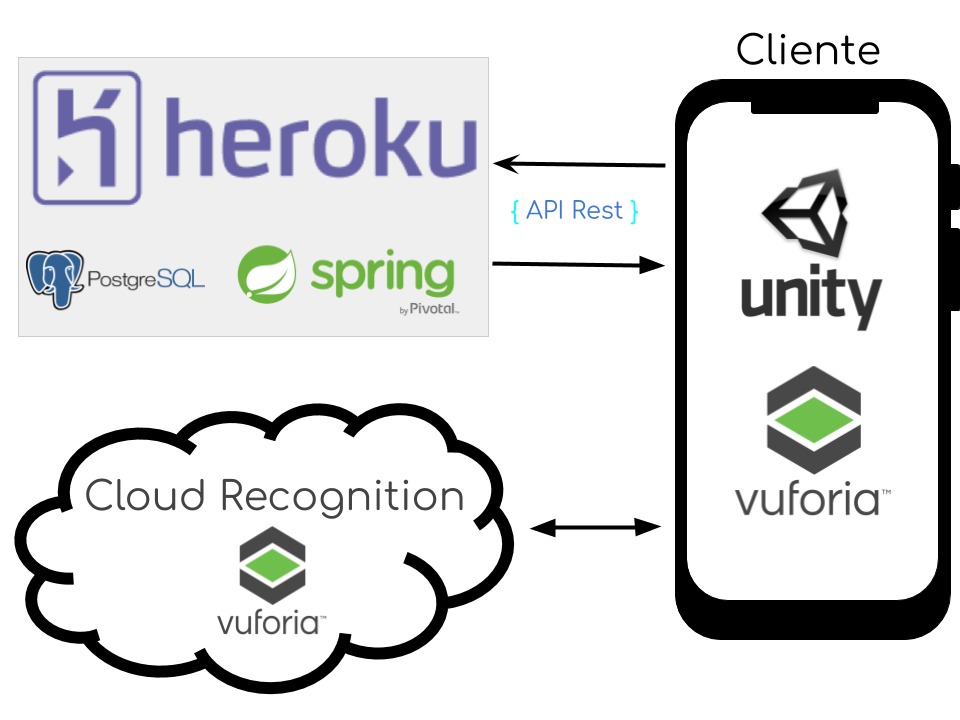
\includegraphics[width=6in]{figures/Arquitectura.png}
    \caption{Arquitectura}
\end{figure}
\section{Servidor}
\label{makereference4.2}
Nuestro servidor está programado en \textbf{Java}, usando el framework \textbf{Spring} para la creación de una \textbf{API Rest} que mediante peticiones \textbf{HTTP} y una base de datos relacional en \textbf{PostgreSQL} nos proporcionará
toda la información necesaria para alimentar de datos a nuestro cliente. El servidor necesita ser desplegado para que la aplicación pueda tener un uso real por lo que conseguimos desplegarlo de forma gratuita en \textbf{Heroku}, que además ofrece
facilidades para desplegar un servidor creado mediante \textbf{Spring}, por lo que nos facilitó el trabajo considerablemente. También se encuentra en el servidor la implementación del sistema de recomendación, con el siguiente punto de acceso \textbf{/recommendations/\{user\}}.
\subsection{Despliegue en Heroku}. 
\label{makereference4.2.1}
Para el despliegue de la aplicación de servidor utilizamos Heroku. Esta plataforma nos ofrece un alojamiento gratuito con las características suficientes para el desarrollo del proyecto.
\begin{figure}[H]
    \centering
    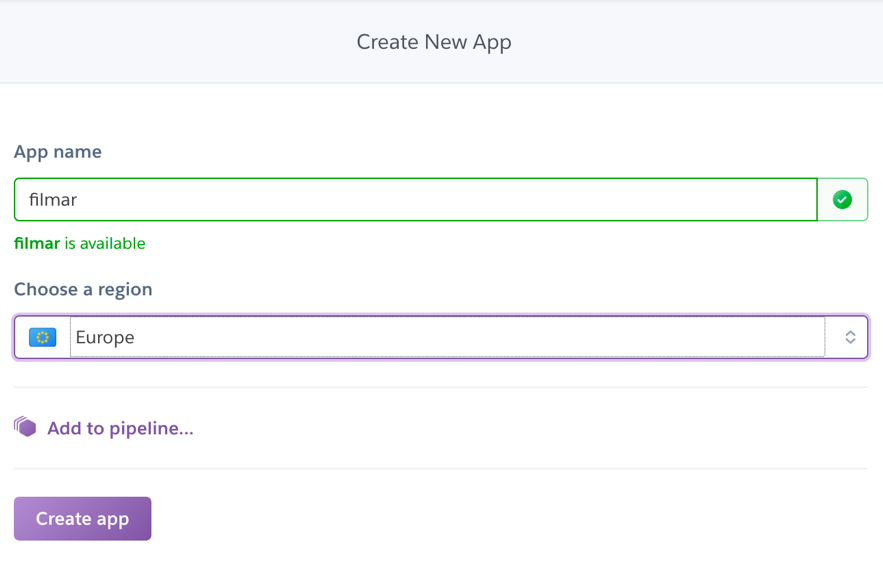
\includegraphics[width=6in]{figures/chapter-4/heroku_1.png}
    \caption{Crear nueva aplicación en Heroku}
\end{figure}
Una vez tenemos una cuenta en la plataforma creamos una nueva aplicación a la cual daremos un nombre como vemos en la figura 4.2 y este nombre a su vez será parte de la URL pública.
\begin{figure}[H]
    \centering
    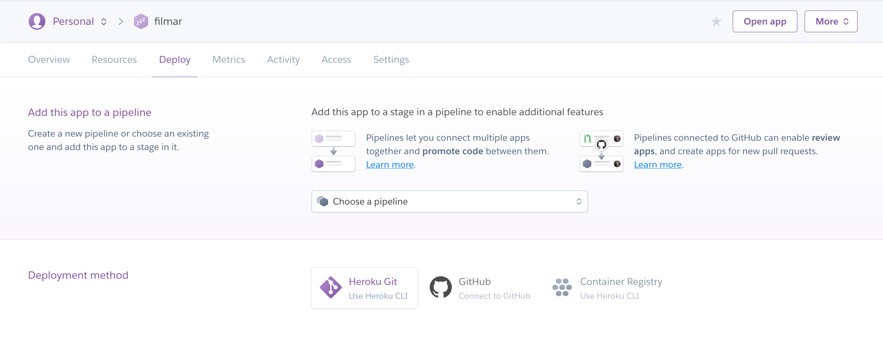
\includegraphics[width=6in]{figures/chapter-4/heroku_2.png}
    \caption{Configuración de la aplicación}
\end{figure}
Cuando creemos la aplicación accederemos a la configuración en la que veremos opciones como en la figura 4.3.
\begin{figure}[H]
    \centering
    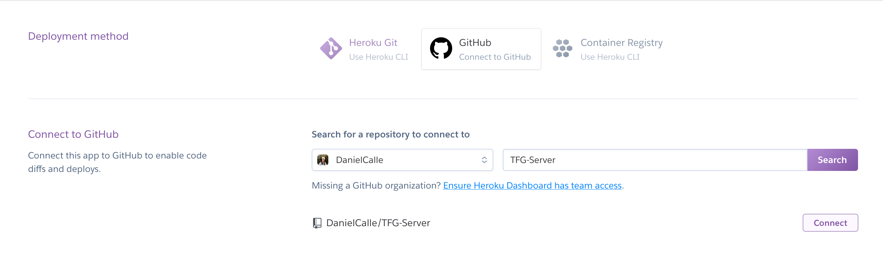
\includegraphics[width=6in]{figures/chapter-4/heroku_3.png}
    \caption{Métodos de despliegue}
\end{figure}
En la figura 4.4 vemos que nos ofrece diversos métodos de despliegue:
\begin{itemize}
    \item Heroku Git
    \item GitHub
    \item Container Registry
\end{itemize}
Elegimos la opción de GitHub que nos proporciona un despliegue fácil y rápido. Tenemos que vincular la cuenta de nuestro GitHub (Importante ser el dueño del repositorio).
\begin{figure}[H]
    \centering
    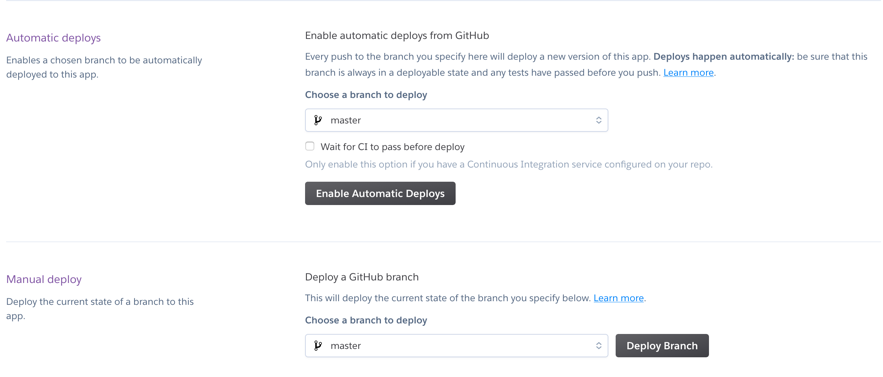
\includegraphics[width=6in]{figures/chapter-4/heroku_4.png}
    \caption{Opciones de despliegue utilizando Github}
\end{figure}
Una vez vinculada la cuenta de GitHub tenemos dos métodos de despliegue como vemos en la figura 4.5. Un método automático para desplegar los cambios de una rama del repositorio que se accionara cada vez que subamos cambios y otro método manual que desplegara solo cuando presionemos el botón. 
Cuando elijamos una de las opciones, la aplicación estará lista para usarse.
\section{Aplicación}
\label{makereference4.3}
Nuestra aplicación está implementada principalmente en \textbf{Android}, las interfaces principales para el uso de los planes, recomendaciones y acceso a la información de las películas guardadas han sido desarrolladas mediante \textbf{Android Studio}. Sin embargo,
la parte del cliente que otorga el gran valor a nuestra aplicación está desarrollada en \textbf{Unity} y el uso de \textbf{Vuforia}, todas las escenas que aparecen al reconocer carteles de películas e imágenes de usuarios fueron implementadas de esta forma. \textbf{Vuforia} además nos ofrece un
servicio de \textbf{Cloud} para el almacenamiento de imágenes, a las cuales les asocia una valoración según lo fácil que le resultará a la aplicación reconocerla y un identificador único (\textbf{UUID}), que es el que usaremos para guardar la distinta información de dicha película o usuario en la base de datos.
La parte de la aplicación realizada en \textbf{Unity}, utiliza una serie de clases de la parte desarrollada en \textbf{Android} para realizar las peticiones al servidor y así poder mostrar información específica cuando se reconoce una cierta imagen.
Al principio hicimos que las dos partes realizaran las peticiones en sus respectivos lenguajes, pero decidimos que sería mejor que el acceso a la capa de datos se realizara por el mismo sitio y así conseguir que las distintas capas estuvieran separadas.
Además, en un principio, las imágenes que mostramos en la parte de \textbf{Android} se almacenan en \textbf{Google Drive} y mediante la librería de \textbf{Picasso} las obtenemos en tiempo de ejecución, esto se ha implementado de esta forma por la misma razón por la que tenemos las imágenes a reconocer en un \textbf{Cloud}.
Finalmente, debido al coste en tiempo de esta operación y tras debatirlo con nuestros directores del Trabajo de Fin de Grado, hemos decidido guardar dichas imágenes en el mismo servidor para su rápida obtención.


Como la mayor parte de la aplicación está implementada en \textbf{Android Studio}, la estructura de ésta se adapta a lo que ofrece el \textbf{IDE}, consistiendo en el flujo de unas actividades y fragmentos que explicaremos a continuación.

\begin{figure}[H]
    \centering
    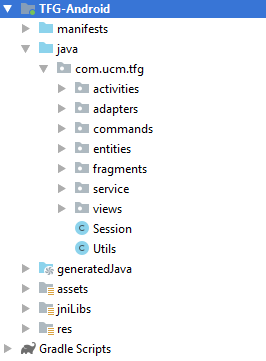
\includegraphics[width=3in]{figures/chapter-4/android_project_structure.png}
    \caption{Estructura de ficheros del proyecto android}
\end{figure}

\subsection{Actividades}
\label{makereference4.3.1}
Son los componentes de la aplicación que representan una pantalla con la que los usuarios pueden interactuar para realizar una determinada acción.

\begin{figure}[H]
    \centering
    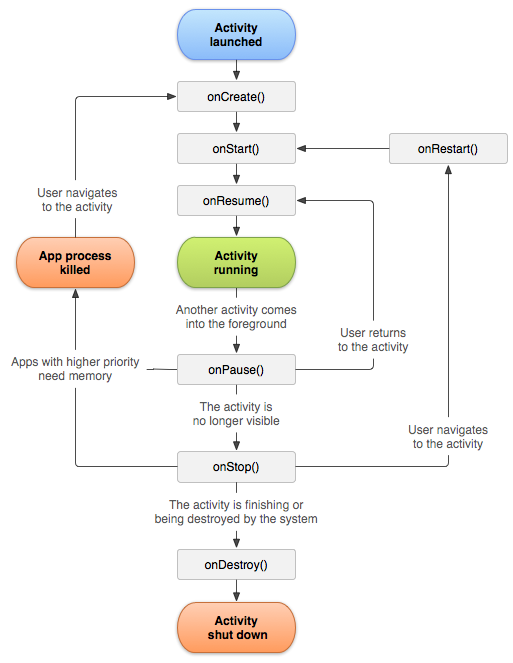
\includegraphics[width=3in]{figures/chapter-4/activity_lifecycle.png}
    \caption{Ciclo de vida de una actividad}
\end{figure}

Entre nuestras actividades podemos destacar dos: 
\begin{itemize}
    \item \textbf{MainActivity:} La primera actividad (actividad principal) que se activa al iniciar la aplicación, la cual comprueba el estado de sesión del usuario, si está logueado se queda en la actividad, y si no, se redirige al usuario a otra actividad (LoginActivity) para que pueda iniciar sesión o registrarse. En la MainActivity se encuentra un paginador (ViewPager) de 3 fragmentos, donde cada fragmento representa las interfaces de planes, recomendaciones y películas guardadas correspondientemente.
    \item \textbf{UnityPlayerActivity:} Se trata de una actividad especial que nos permite comunicar la parte desarrollada en \textbf{Unity} con nuestro proyecto \textbf{Android}. Aquí se encuentran llamadas a funciones desde la parte de Unity, se realizan las órdenes y se devuelven.
\end{itemize} 

\subsection{Adaptadores}
\label{makereference4.3.2} 
Son elementos de manipulación de datos que se aplican a vistas y componentes. En el proyecto se les ha dado mucho uso a las vistas de tipo \textbf{RecyclerView} para representar listas de objetos. Para manejar los datos de cada elemento de la lista, se ha utilizado un \textbf{RecyclerView.Adapter}, el cual manipula cada dato correspondiente a un elemento de la lista. También se han creado otros adaptadores, como uno para manejar tres fragmentos dentro de una actividad, como hemos dicho anteriormente al describir la actividad principal (MainActivity).

\subsection{Comandos}
\label{makereference4.3.3}
Aquí se encuentran todos los elementos relacionados con el patrón comando y ha sido diseñado para realizar la conexión con la parte del proyecto desarrollado en Unity.

\begin{figure}[H]
    \centering
    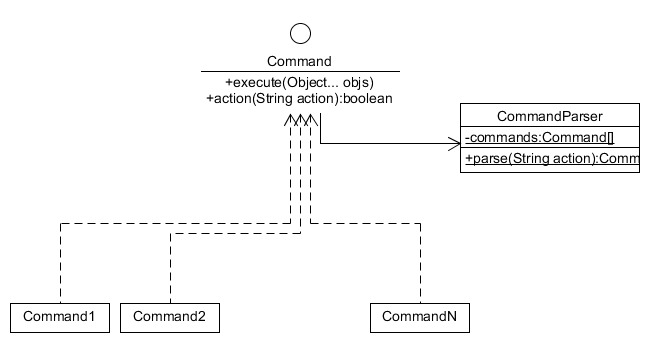
\includegraphics[width=3in]{figures/chapter-4/command_pattern.png}
    \caption{Patrón comando}
\end{figure}

Este patrón permite solicitar una operación a un objeto sin conocer realmente el contenido de esta operación, ni el receptor real de la misma. Para ello se encapsula la petición como un objeto, con lo que además facilita la parametrización de los métodos.

La implementación de este patrón consiste en crear una interfaz en la cual las demás clases (comandos) la implementan. La interfaz tiene dos funciones: 
\begin{itemize}
    \item  \textbf{execute} para ejecutar la tarea.
    \item  \textbf{action} para comprobar si este comando es el indicado para ejecutar la tarea. 
\end{itemize} 
Por otro lado, tenemos una clase llamada \textbf{CommandParser}, encargada de buscar el comando apropiado para su ejecución.

\subsection{Entidades}
\label{makereference4.3.4}
Todos los modelos de datos que podemos recibir del servidor como planes, películas, usuarios, etc. Son representados por entidades en nuestro proyecto de \textbf{Android}, con los mismos atributos que tienen sus entidades correspondientes en el servidor.

\subsection{Fragmentos}
\label{makereference4.3.5}
Representan un comportamiento o una parte de la interfaz de usuario en una actividad.

\begin{figure}[H]
    \centering
    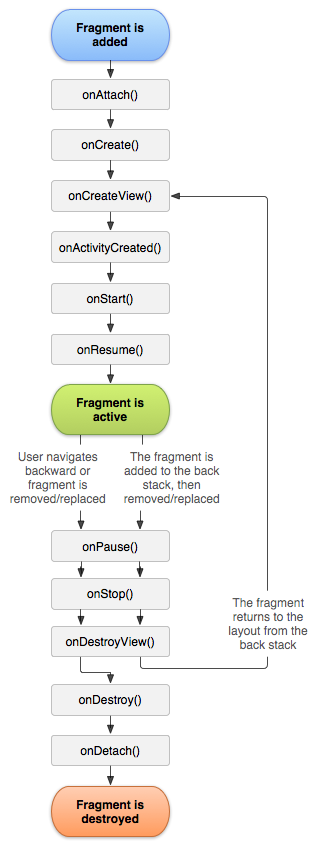
\includegraphics[width=3in]{figures/chapter-4/fragment_lifecycle.png}
    \caption{Ciclo de vida de un fragmento}
\end{figure}

Se utilizan para formar una vista compuesta de paginación en una actividad. 

\subsection{Servicios}
\label{makereference4.3.6}
Se trata de un conjunto de clases que solo poseen métodos estáticos para llevar a cabo peticiones \textbf{HTTP} al servidor. Se ha creado una clase genérica para la creación y llamada de peticiones \textbf{HTTP}, se ha diseñado de manera que las respuestas se devuelvan en forma de \textbf{callback} para un uso más sencillo.

\subsection{Vistas}
\label{makereference4.3.7}
Entre los componentes que ofrece \textbf{Android} hay algunas funcionalidades que no soporta. Entonces se crean componentes personalizados para satisfacer a estas funcionalidades:
\begin{itemize}
    \item \textbf{AnchorVisibilityBehavior:} Implementa un comportamiento el cual aplicado a una vista determinada, genera el comportamiento deseado. En este caso el comportamiento es la visibilidad que tiene algunas vistas colocadas en un toolbar (depende de su altura). 
    \item \textbf{CustomViewPager:} ViewPager es lo que se usa en el MainActivity para colocar los tres fragmentos. Se crea esta clase para desactivar la acción de poder pasar los fragmentos mediante deslizamiento.
    \item \textbf{ExpandableTextView:} Es una clase que extiende de un TextView, se le añade un método para que cuando haya mucho texto, se pueda acortar. Además dispone de un botón para expandir.
\end{itemize} 

\section{Dificultades encontradas}
\label{makereference4.4}
A continuación, mostraremos una lista de todas las dificultades encontradas a la hora de implementar nuestra aplicación:
\begin{itemize}
    \item Diseño de las interfaces para que fueran familiares e intuitivas para el usuario.
    \item Desconocimiento del entorno de desarrollo y peculiaridades del desarrollo de aplicaciones en \textbf{Android}.
    \item Incompatibilidad de realización de peticiones \textbf{HTTP} en ciertas versiones de \textbf{Android}.
    \item Problemas a la hora de intentar desplegar el servidor de forma correcta para que fuera accesible siempre.
    \item Poca familiaridad con el uso de \textbf{Unity} y el lenguaje \textbf{C\#} para realizar la parte de realidad aumentada.
    \item Caducidad de las licencias gratuitas para el uso del \textbf{Cloud} de \textbf{Vuforia}.
    \item Primera vez usando el framework de \textbf{Spring} para la realización de una \textbf{API Rest}.
    \item Comunicación entre la parte cliente en \textbf{Android} y el servidor.
    \item Comunicación entre la parte cliente en \textbf{Unity} con la parte cliente en \textbf{Android}.
    \item Rendimiento en cuanto al reconocimiento de ciertas imágenes, sobre todo de personas, debido a la calidad de las mismas. El \textbf{Cloud} de \textbf{Vuforia} no las reconoce tan fácilmente como las de carteles de películas.
    \item Almacenamiento de imágenes en \textbf{Google Drive} y su obtención desde \textbf{Android} y \textbf{Unity}, junto con el retardo que esto produce.
    \item Dificultades para configurar inicialmente el proyecto de \textbf{Unity} para que éste funcionase con el \textbf{Cloud} de \textbf{Vuforia}.
    \item Incompatibilidades con las nuevas actualizaciones de \textbf{Unity}.
    \item Parte de la documentación de \textbf{Vuforia} contiene elementos de \textbf{Unity} y \textbf{Vuforia} de versiones desfasadas.
\end{itemize}
\section{Herramientas de trabajo}
\label{makereference4.5}
Las distintas herramientas de trabajo que hemos decidido usar para que el trabajo realizado fuera más eficiente son las siguientes:
\begin{itemize}
    \item \textbf{Telegram:} hemos usado esta aplicación de mensajería para poder comunicarnos entre todos los miembros pertenecientes al proyecto, ya fuera para la sugerencia de ideas o que un bot de \textbf{Github} nos avisara de los cambios en los distintos repositorios que hemos creado. 
    \item \textbf{Slack:} esta otra herramienta de comunicación nos ha permitido crear canales específicos para cada parte de nuestro proyecto y así poder clasificar las conversaciones que teníamos por temas, por ejemplo, tenemos un canal para hablar solo de la parte backend, otro para hablar de la parte de realidad aumentada, etc. Cosa que \textbf{Telegram} no nos permitía y resultaba lioso encontrar ciertos temas o puntos de nuestras conversaciones. 
    \item \textbf{Trello:} nos ha servido como apoyo para realizar nuestros sprints, \textbf{Trello} nos ofrece la posibilidad de crear un tablero para escribir tareas a modo de post-it y asignarlas a usuarios que estén dentro del tablero, así sabemos qué tipo de tareas ha realizado o está realizando cada miembro en todo momento.
    \item \textbf{GitHub:} todos nuestros repositorios están en \textbf{GitHub}, lo que nos permite subir cambios y trabajar en paralelo en distintas ramas, agilizando así nuestro trabajo y otorgándonos un control de versiones muy estable.
    \item \textbf{Visual Studio Code:} utilizamos este editor de código junto con la extensión de \textbf{LaTeX Workshop} para escribir la memoria en \textbf{LaTeX}.
    \item \textbf{Android Studio:} usamos este IDE para construir la aplicación \textbf{Android} que además nos dota de herramientas de depuración.
    \item \textbf{Google Drive:} almacenamiento en la nube donde tenemos toda la información relevante para el TFG.
    \item \textbf{Heroku:} plataforma en la que desplegamos nuestra aplicación de servidor.
    \item \textbf{Unity:} Utilizamos esta plataforma de desarrollo para construir la parte de la aplicación relacionada con \textbf{Realidad Aumentada}.
    \item \textbf{Visual Studio:} Utilizamos Visual Studio para codificar los scripts en \textbf{C\#} necesarios para el funcionamiento de la parte de Realidad Aumentada en Unity.
    \item \textbf{Postman:} aplicación para el envío de peticiones HTTP REST, que utilizamos para depurar los servicios de \textbf{Spring}.
    \item \textbf{MockFlow:} herramienta online para el diseño de mockups, nosotros la utilizamos para el diseño de las vistas de la aplicación \textbf{Android}.
\end{itemize}
